\documentclass[14pt]{extarticle}
\usepackage{amsmath}
\usepackage{amssymb}
\usepackage{gvv}
\usepackage{graphicx}
\usepackage{tfrupee}
\title{\textbf{5.8.3}}
\author{\textbf{Aditya Mishra-EE25BTECH11005}}
\date{October 10, 2025}

\begin{document}
\maketitle

\section*{Question}
5 pencils and 7 pens together cost \rupee50, whereas 7 pencils and 5 pens together cost \rupee46.  
Find the cost of one pencil and that of one pen.

\section*{Solution}
Let the cost of one pencil be \(x\) and the cost of one pen be \(y\) (both in rupees).  

\begin{align}
5x + 7y &= 50 \\
7x + 5y &= 46
\end{align}

Thus, the word problem is converted into a system of linear equations:
\begin{align}
\begin{cases}
5x + 7y = 50 \\
7x + 5y = 46
\end{cases}
\end{align}

Forming the augmented matrix:
\begin{align}
\augvec{2}{1}{5 & 7 & 50 \\ 7 & 5 & 46}
\end{align}

Perform row operations to reduce to row echelon form:
\begin{align}
\augvec{2}{1}{5 & 7 & 50 \\ 7 & 5 & 46}
&\xrightarrow{R_2 \rightarrow R_2 - \frac{7}{5}R_1}
\augvec{2}{1}{5 & 7 & 50 \\ 0 & -4.8 & -24}
\end{align}

From the second row:
\begin{align}
-4.8y &= -24 \implies y = 5
\end{align}

Substitute into the first row:
\begin{align}
5x + 7y &= 50 \implies 5x + 35 = 50 \implies x = 3
\end{align}

Thus, the cost of one pencil is \rupee3 and the cost of one pen is \rupee5:
\begin{align}
\boxed{
\vec{x} = \myvec{3 \\ 5}
}
\end{align}

\section*{Plot}
\begin{figure}[!h]
    \centering
    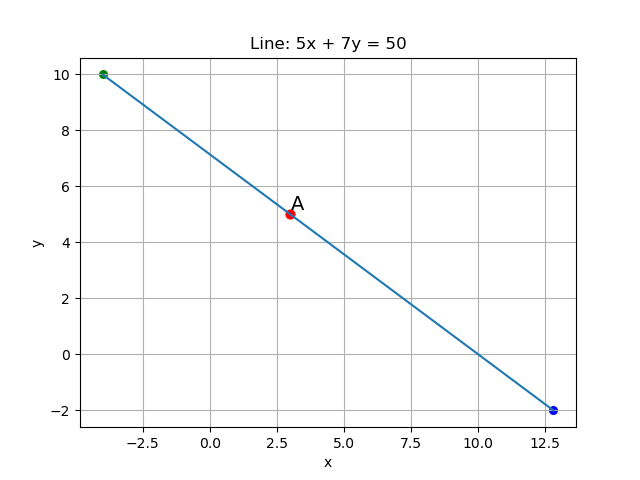
\includegraphics[width=1.2\columnwidth]{Figs/Figure_1.png}
\end{figure}

\end{document}

